\section{Experiments} 
\todo{Add axis labels to all graphs}

\dmcmt{ Would it be a good idea to have an applications and experiments section,
    where we phrase each experiment as a potential application of our
    abstraction framework? That way, we can dwell a bit more on why such an
application makes sense. In sec 3.5 we have had to write something generic to
various applicaitons, this will give us some opportunity to flesh that out. Time
and space may be a concern.}

We have implemented our method in python\footnote{The entirety of the code,
    networks, datasets, and properties utilized in our evaluation will be made
    available via a publicly hosted code repository in the
camera ready version.}, utilizing the NumPy library for linear algebra
operations and the SciPy library for an implementation of \hcluster.
We have used a linkage-matrix based data structure similar to the one used in
SciPy to store the tree, and have precomputed and cached several
operations that may need to be repeated every refinement iteration. This allows
us to quickly perform the merge and split operations and calculate the
scores (Section \ref{s:refinement}), without having to do (relatively)
expensive tree traversal operations in each iteration of the abstraction
refinement loop. 

Using this implementation, we have performed three sets of experiments to
demonstrate the usefulness of our technique. In several safety-critical
settings, such as medical diagnosis and collision detection, where \dnn are
deployed as classifiers, false negative classification with respect to some
classes is highly undesirable. In the first set of experiments, we show that
our abstraction technique can be leveraged to obtain effective compression of
\dnn in such settings, with a guarantee that the compression does not introduce
any new false negative classifications (Section \ref{s:exp-mnist-comp}). In our
second set of experiments, we demonstrate how our technique may be used to
obtain abstract networks with the aim of proving a given property, plotting the
number of spurious counterexamples introduced as the size of the abstract
network reduces (Section \ref{s:exp-mnist-rob}). Finally, in the last set of
experiments, we show how our technique may be used in a CEGAR loop
\cite{cegar-nn} to verify the \acasxu properties (Section \ref{s:acas-verif}).
We utilized \abcrown as the solver in the backend for these experiments. 

If the \abs produced has multiple neurons with the exact same set of incoming
edges in the same layer, these neurons compute the same function and are
redundant. Therefore, as an added optimization step, we safely \textit{re-merge}
them by taking the sum of the outgoing edges. Note that this does not change the
behavior of \abs.

\todo{Make the following proper}
The experimental results in Tables
\ref{t:mnist-compr-summary}, 
\ref{t:acas-ncex}, \ref{t:acas-verif} and Figures \ref{f:acas-ncex-samples},
\ref{f:acas-ncex-pgd}, \ref{f:acas-verif-ref},
\ref{f:mnist-class} were
run on a machine running on an Intel(R) Core(TM) i7-9700K with 8 CPUs running at
3.60GHz, having 16 GB RAM and running Ubuntu 22.04 LTS. The results in
Figures \ref{f:mnist-prop-samples}, Figures \ref{f:mnist-prop-pgd} and Table
\ref{t:mnist-prop-summary} were produced on a 
machine running on an Intel(R) Core(TM) i7-13700 with 24 CPUs running at
5.20GHz, having 32 GB RAM and running Ubuntu 23.10.

\subsection{Compression with Guarantees on Critical Classes}
\label{s:exp-mnist-comp}

Safety-critical analysis of neural networks is highly sensitive to the size of
the network. While several neural network compression techniques exist 
\cite{dnn-compression}, they do not provide formal guarantees 
connecting the behavior of the compressed network and the original network.
Similarly, although existing semantic abstraction techniques have been proposed
as a way to compress neural networks, the guarantees provided by such 
techniques are of an empirical nature \cite{lin-comb-abs-jan}.
This lack of guarantees also limits the usefulness of these compression
techniques as optimization steps when deploying a safety-critical network in a
resource-constrained environment. 

\begin{wrapfigure}{r}{0.5\textwidth}
    \vspace*{-1cm}
    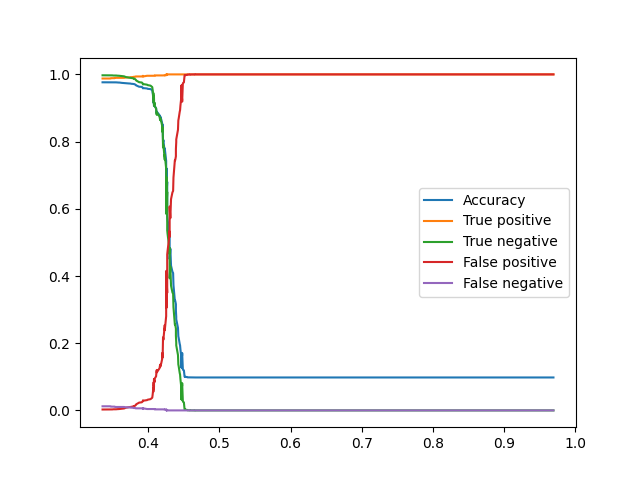
\includegraphics[scale=0.4]{figs/mnist-compr-4-256-samples.png}
    \caption{Accuracy and True/False Positive/Negative Rates vs Reduction Rate
        plot for \mnist of size $4 \times 256$ with critical class 0. Refinement
    done via the \emph{Score} strategy. In all graphs the Y-axis shows
    true/false negative/positive rates (see legend) and the X-axis shows
    reduction rates.  \todo{Add labels on graphs here} }
    \label{f:mnist-class}
    \vspace*{-1cm}
\end{wrapfigure}

Our theoretical framework for abstraction allows us to produce compressed
networks with the formal guarantee that the abstraction process will not
introduce any new \emph{false negatives} with respect to a certain
\emph{critical output class} $c$. Specifically, if \cnc classifies an input
$\vct{x}$ as $c$, \abs is also guaranteed to classify $\vct{x}$ as $c$. This is
useful in several safety critical domains, including medical diagnosis and
collision detection, where the critical classification would say that a patient
is disease free, or that a situation will not lead to a collision. In such
scenarios, obtaining a false negative (that is, \abs claiming a
patient is disease free or that a situation would not lead to a collision while
\cnc does not) is highly undesirable. 

We do this by marking the output neuron $n_c$ corresponding to the critical
class $c$ in the output layer as \inc, and all other neurons in the output layer
as \dec.  Then, for any input that \cnc classified into
the critical class, $n_c$ will have the largest value in the
output layer, and as it has been marked as \inc, it will continue to have the
largest value in the output layer for \abs as well. Thus, the
abstract network will also classify this input as critical. 

However, the \abs obtained via this method may introduce
\emph{false positives}. These correspond to producing false alarms (\abs
produces a diagnosis of a disease, or flags a collision when \cnc does not), and
do not affect safety adversely. Each such input producing a false positive
would be a \gencex which we may try to eliminate via an abstraction refinement
loop.

We demonstrate the effectiveness of our abstraction method as a
compression-with-guarantees technique via some experiments on \mnist. We set the
class `0' as the critical class. Then, starting with the fully merged network,
we iteratively perform refinements while measuring the accuracy, false/true
positive/negative rates. We perform these experiments with four strategies of
selecting the culprit neuron $\gamma$ mentioned in Section
\ref{s:finding-gamma}.

Figure \ref{f:mnist-class} shows some typical plots of the true/false
negative/positive rates (y-axis) against reduction rate (x-axis). Note that the
reduction rate plotted is with respect to the size of the network obtained after
\inc-\dec splitting. While this may mean that the \abs produced may be greater
in size than the original network, note that in such an \abs each neuron can be
cleanly classified as \inc or \dec with respect to a property of interest, which
may make formal analysis simpler. Indeed, it has been seen that such \abs, while
larger, may be easier to verify \cite{cegar-nn}. \dmcmt{Can this section be
shortened}

We notice that, as guaranteed by the theory, the false negative rate never
increases, even as the reduction rate approaches close to $100\%$. In fact, the
false negative rate improves, as some of the points that are going
to be newly classified as positive may in fact be true positives.  
However, as discussed before, we do pay for the compression by introducing false
positives, which we see in the graph. 

We also find in the graph that there is a
small window of reduction rate values where almost all of the improvement in the
false positive rate occurs. This indicates that we are eventually able to make 
significant improvements in the false positive rate while sacrificing the
reduction rate as little as possible. Thus, our technique is able to use
semantic information to order and undo merge operations in an optimal way.

\begin{table}
\begin{tabular}{|c|c|c|c|c|}
\hline
Net Size     & $\gamma$ Selection & Reduction & False Positives & Steps  \\ 
\hline
$2\times256$ & Random             & 50.0 \%   & 0.2  \%         &  923   \\  
$4\times256$ & Random             & 50.0 \%   & 0.2  \%         & 1917    \\ 
$6\times256$ & Random             & 50.0 \%   & 0.2  \%         & 2999    \\ 
$2\times256$ & Score      & 45.7 \%   & 0.3  \%         &  326    \\ 
$4\times256$ & Score      & 38.7 \%   & 2.2  \%         & 1037    \\ 
$6\times256$ & Score      & 45.5 \%   & 0.2  \%         & 2425    \\ 
\hline
\end{tabular}
\caption{Summary of \mnist compression Results}
\label{t:mnist-compr-summary}
\end{table}

Table \ref{t:mnist-compr-summary} summarizes the results from running all the
compression experiment on all the \mnist network via various strategies for
selecting $\gamma$. For each instance, we report the best reduction
rate achieved (column `Reduction') for a network whose false positive rate was
close to the best false positive rate seen (Column `False Positives')
throughout the refinement process. Intuitively, these two columns characterise
the quality of the \abs obtained. The `Steps' column shows the
number of refinement steps it took to arrive at these networks, and represents
how much effort the search for the \abs took. \footnote{ Note that we currently do
not stop our refinement loop at the precise point where this network is produced
but may continue to refine beyond this point. \dmcmt{Is it okay to keep as a
footnote? Can we remove this point entirely? }}

Overall, we find that the quality of the networks are similar across the two
$\gamma$ selection strategies, while the number of steps
taken to arrive at the network is lower for \emph{Score} compared to the Random
baseline. This would indicate that the strategy used to select $\gamma$ only
affects the effort needed to do the search, not the quality of \abs obtained at
the end of the search. This is in contrast with other structural abstraction
refinement base techniques like \cite{cegar-nn,cegarette,cleverest-nn}, where
the choice of which abstract node to refine at each step plays a critical role
on both the size and the amount of over-approximation in the network. \dmcmt{Can
anything at all be said about the quality of the \abs here, without a baseline
to compare to?}

\subsection{Eliminating Spurious Counterexamples}
\label{s:exp-mnist-rob}

In this section, we explore how well our abstraction refinement process is able
to remove spurious counterexamples. We start with the abstract network and
iteratively perform refinements, measuring the number of spurious
counterexamples at each step. 

\begin{figure}

    \begin{subfigure}{0.475\linewidth}
        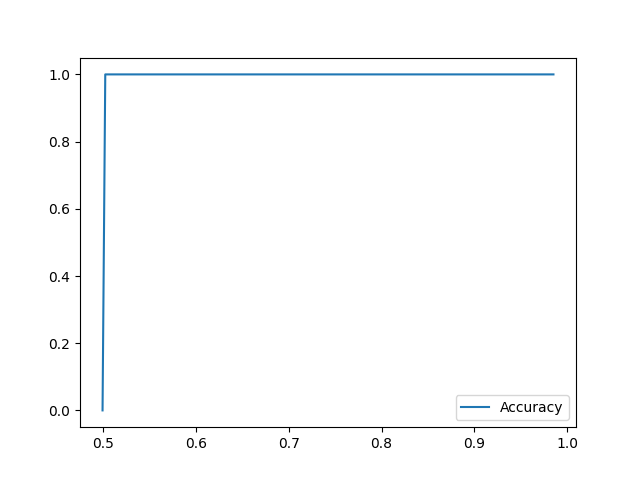
\includegraphics[scale=0.4]{figs/mnist_2_256_prop_0_0.03_samples.png}
        \caption{}
        \label{f:mnist-prop-samples}
    \end{subfigure}
    \begin{subfigure}{0.475\linewidth}
        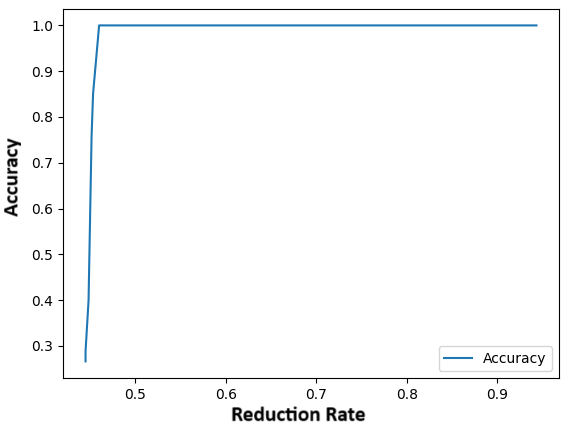
\includegraphics[scale=0.4]{figs/acas_ncex_5_8_3_samples.png}
        \caption{}
        \label{f:acas-ncex-samples}
    \end{subfigure}

    \caption{
        Spurious counterexample vs Reduction Rate plot for \mnist of size $2
        \times 256$ with $\epsilon$-Robustness property are given in 
        \ref{f:mnist-prop-samples}, and for \acasxu
        network 5-8, property 3 in \ref{f:acas-ncex-samples}.
        $\gamma$ selection is via \emph{Score}. \todo{Label axis on graph}
    }
    \label{f:ncex}
\end{figure}

We experimented with two sets of networks and properties: \mnist with
adversarial robustness properties and \acasxu with the properties from
\cite{reluplex}. For each, we tried the 2 strategies for choosing $\gamma$ from
Section \ref{s:finding-gamma}.
Figure \ref{f:ncex} shows some typical plots
for these experiments. Here, the x-axis measures the reduction rate with respect
to the \inc-\dec split networks, and the y-axis is the rate of true
counterexamples within a random sample. A low y-axis value indicates a good
abstraction.

Similar to Section \ref{s:exp-mnist-comp}, we see that there is a small window
of reduction rate values where most of the improvement in over-approximation
occurs. As before, we believe that this is evidence that we are able to use
semantic information and undo merge operations optimally.

\begin{table}
\parbox{0.60\textwidth}{
\begin{tabular}{|c|c|c|c|c|}
    \hline
    Net Size     & $\gamma$ Selection  & Reduction & Cex. Rate & No. Steps \\
    \hline
    $2\times256$ & Random              & $49.1\%$  & $  0\%$  & $ 899$    \\
    $4\times256$ & Random              & $49.6\%$  & $  0\%$  & $1929$    \\
    $6\times256$ & Random              & $49.7\%$  & $  0\%$  & $2818$    \\
    $2\times256$ & Score               & $50.3\%$  & $  0\%$  & $  27$    \\
    $4\times256$ & Score               & $49.9\%$  & $  0\%$  & $ 648$    \\
    $6\times256$ & Score               & $47.9\%$  & $  0\%$  & $1199$    \\
    \hline
\end{tabular}
\caption{Summary of \mnist Results on a single robustness property }
\label{t:mnist-prop-summary}
}
\quad
\parbox{0.30\textwidth}{
\begin{tabular}{|c|cc|}
\hline
$\gamma$ Selection  & Score   & Random  \\
\hline
Reduction  & 45.5\%  & 50.9\%  \\
Sp. Cex.   & 13.0\%  & 3.6\%   \\
Avg. Steps & 294.111 & 512.011 \\
\hline
\end{tabular}
\caption{Summary of \acasxu, $\gamma$ selection is along columns.}
\label{t:acas-ncex}
}
\vspace{-1cm}
\end{table}

Table \ref{t:mnist-prop-summary} summarizes our observations for \mnist, and
\ref{t:acas-ncex} for the \acasxu networks. The meaning of the columns are
exactly the same as in Table \ref{t:mnist-compr-summar} in Section
\ref{s:exp-mnist-comp}. In fact, we see that both $\gamma$ selection methods
arrive at \abs with similar reduction rates. For the \mnist networks, both
methods are able to eliminate all counterexamples.  Again, we see that
\textit{Random} takes more steps to arrive at the \abs. Thus, this reinforces
our intuition that $\gamma$ selection mainly affects the number of refinement
steps taken by the search, and does not strongly affect the quality of \abs
found.

\subsection{Verification of \acasxu}
\label{s:acas-verif}
\todo{If adv \cite{reluplex,cegar-nn} results are in, include them}
\dmcmt{Push to front}

In this set of experiments, we demonstrate the effectiveness of our abstraction
technique for verification of neural network queries on the \acasxu set of
benchmarks. To do so, we set up a \cegar loop (Section \ref{s:abs-ref-fw}) using
our abstraction technique, where on each \abs generated we call a neural network
solver. If the solver returns a spurious counterexample, we use
that as $\vct{\beta}$ to refine our network according to Section
\ref{s:refinement}.  

For these experiments, we have used \neuralsat as the solver. 
We compare our abstraction framework with an existing \cegar framework proposed
in \cite{cegar-nn}. 
\footnote{We have used a faithful re-implementation of this framework that
follows exactly the procedure in the paper, with the only distinction being that
the call to verify the \abs obtained in each iteration is sent to an instance of
the \neuralsat solver as opposed to \marabou. \dmcmt{Is this okay?}}. We set a
timeout of 200 seconds for each instance in the benchmark and for both the
our technique and the existing work \cite{cegar-nn}.

\begin{table}
%\footnotesize
\begin{tabular}{ |c|c|c|c| }
\hline
Method                   & No. Safe & No. Unsafe & No. Timeout \\ 
\hline
Ours                     &   121       & 43       & 16    \\
Existing \cite{cegar-nn} &   118       & 43       & 19    \\
\hline                                                                
\end{tabular}
\caption{Summary of \acasxu verification. }
\label{t:acas-verif}
\end{table}

Table \ref{acas-verif} summarizes the results on these benchmarks. We find that
using our framework, we are able to perform better than the existing \cegar
approach \cite{cegar-nn}, verifying more networks to be safe.

\begin{figure}
    \centering
    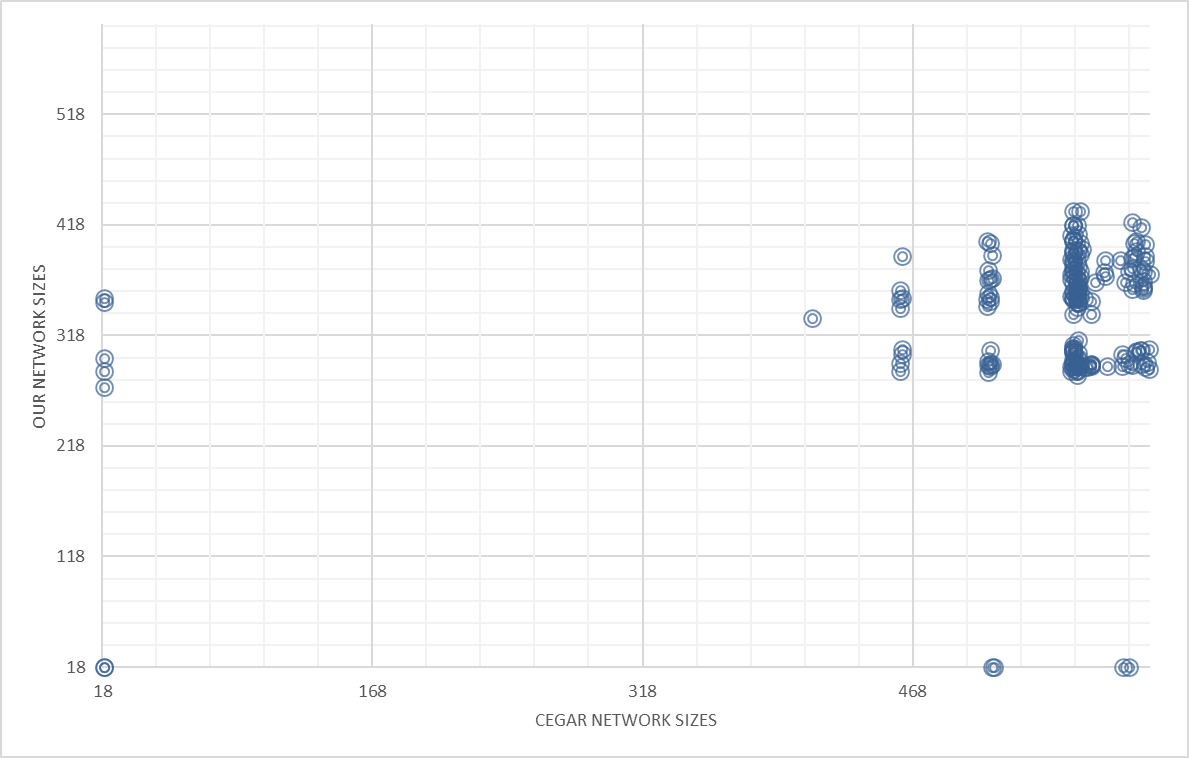
\includegraphics[scale=0.25]{figs/scatter-cegar-our-nerualsat.png}
    \caption{Scatter plot of network sizes produced by our framework vs existing
    work \cite{cegar-nn} \todo{Add diagonal line}}
    \label{f:scatter-netsizes}
\end{figure}

For each framework, we collected the final \abs at the end of the \cegar
iterations, for which either the property can be proved to be safe, or 
the solver is able to find an actual counterexample, or the solver times out.  
Figure \ref{f:scatter-netsizes} shows a scatter plot comparing the sizes of these final \abs
obtained by our framework and by existing work \cite{cegar-nn} for each instance
in the benchmark.
We find that compared to the existing techniques, we are explore smaller
\abs that are effective at proving or disproving the property in question. This
shows that using semantic information to guide the \cegar process can
effectively find more efficient abstractions than the existing technique.

Note that in our experiments, we found that the time taken by both our \cegar
approach and the existing \cegar approach \cite{cegar-nn} was more than what the
\neuralsat solver takes for the \acasxu benchmarks. However, while we would
expect the solver call times to exponentially scale with network size, the
overheads from the abstraction procedure will not scale exponentially. Thus, for
larger and larger benchmarks, being able to find smaller \abs will produce a
significant difference in times. Furthermore, we believe that a verified \abs is
useful beyond verifying a single property - it may be used for other related
queries, or may be useful as a safely deployable compressed network.
\dmcmt{Is this okay?} 

\dmcmt{Do we need the following?}
In general, we have
observed that solver times are highly dependent on solver configuration and the
benchmark rather than on size. Thus, it may seem that the effort needed to
verify a network is dependent on other factors than simply the size of the
network. While this may be interesting to explore in future work, we nonetheless
argue that network size is a relevant metric. This is because, even as more and
more solvers are designed and optimized for various kinds of networks, the
underlying worst-case performance will almost certainly remain exponential in
the size of the network \cite{reluplex}. \todo{Modify if
we get final call times from cegar-nn}.

